\documentclass[runningheads]{llncs}

\usepackage{iftex}
\ifPDFTeX
  \PackageError{short}{This manuscript must be built with XeLaTeX}{}
\else
  \usepackage{fontspec}
\fi
\usepackage{amsmath,amssymb}
\usepackage{booktabs}
\usepackage{graphicx}
\usepackage{xcolor}
\usepackage{hyperref}
\renewcommand\UrlFont{\color{blue}\rmfamily}
\urlstyle{rm}
\graphicspath{{figures/}}
\emergencystretch=1.5em

% GENERATED FILE: accepted confirmation evidence only. DO NOT EDIT.
% Raw confirmation rows and oracle diagnostics are outside this renderer.
\newif\ifshortresultsconfirmed
\shortresultsconfirmedtrue
\newcommand{\ShortUnavailable}{\textsc{Confirmed results available}}
\newcommand{\ShortResult}[1]{\PackageError{short_results}{Unknown result selector `#1'}{Use only generated named result macros or tables.}}
\newcommand{\ShortAdverseNullRetained}{true}
\newcommand{\ShortConfirmationAnalysisSHA}{\texttt{60550c2b09295928ed3c27113a4ca8955f12228e4b64d0af5432ca9cf9b33ffb}}
\newcommand{\ShortConfirmationResultSHA}{\texttt{a7497eaa80d8d7260cc12a603a2240364184b04574260dee2bc685ead7333cf8}}
\newcommand{\ShortConfirmationPayloadSHA}{\texttt{d1b584b99fff4801645e75af96b26c37dbff092ed2bcd666128f6a512864d8e5}}
\newcommand{\ShortCalibrationSelectionSHA}{\texttt{8f390f1969bafee5c6aed760332128a421da24b5e11282394e4f7c7eeb1f45da}}
\newcommand{\ShortProtocolSHA}{\texttt{754cdb90a592003dbf5319535ebb476d2baebe19f07a67eaab562ba99c3f575e}}
\newcommand{\ShortEffectCell}[3]{$#1\,[#2,#3]$}
\newcommand{\ShortClusteringClaimGate}{blocked}
\newcommand{\ShortPriorityClaimGate}{blocked}
\newcommand{\ShortDuplicateClaimGate}{eligible}
\newcommand{\ShortDispatchEvidenceGate}{blocked}
\newcommand{\ShortProductConfiguration}{config.product\_louvain.097}
\newcommand{\ShortAdditiveConfiguration}{config.additive\_louvain.084}
\newcommand{\ShortSTDBSCANConfiguration}{config.st\_dbscan.056}
\newcommand{\ShortHDBSCANConfiguration}{config.hdbscan.007}

\newcommand{\ShortClusteringResultsTable}{%
\begin{table}[t]
\centering\small
\caption{Clustering descriptives over 40 paired master seeds. FD, NR, and Review denote false destinations per 100 reports, noise rejection, and review items per 100 reports; no adverse or null result is suppressed.}
\label{tab:short-clustering-results}
\begin{tabular}{llrrrr}
\toprule
Regime & Method & ARI & FD & NR & Review \\
\midrule
ID & Product & 0.73 & 4.98 & 0.00 & 16.53 \\
ID & Additive & 0.90 & 4.89 & 0.00 & 9.91 \\
ID & ST-DBSCAN & 0.85 & 0.00 & 0.97 & 9.66 \\
ID & HDBSCAN & 0.85 & 0.07 & 0.41 & 6.95 \\
\midrule
OOD & Product & 0.36 & 17.13 & 0.00 & 45.35 \\
OOD & Additive & 0.46 & 13.02 & 0.00 & 37.53 \\
OOD & ST-DBSCAN & 0.56 & 0.41 & 0.88 & 43.20 \\
OOD & HDBSCAN & 0.56 & 1.18 & 0.39 & 31.18 \\
\bottomrule
\end{tabular}
\end{table}%
}

\newcommand{\ShortPriorityDispatchResultsTable}{%
\begin{table}[t]
\centering\footnotesize
\setlength{\tabcolsep}{2pt}
\caption{Paired headline effects with 95\% bootstrap confidence intervals. Every $\Delta$ is improvement-oriented, so positive favors the revised heuristic; adverse and null effects remain visible. Dispatch values first average the three locked scenarios within each master seed; H is harm and D is deadline-miss percentage points.}
\label{tab:short-priority-dispatch-results}
\begin{tabular}{@{}llcc@{}}
\toprule
\multicolumn{4}{l}{\textit{Panel A: Priority alignment (revised minus baseline)}} \\
\multicolumn{2}{l}{Baseline} & ID $\Delta$NDCG@5 & OOD $\Delta$NDCG@5 \\
\midrule
\multicolumn{2}{l}{Legacy} & \ShortEffectCell{-0.09}{-0.12}{-0.06} & \ShortEffectCell{-0.07}{-0.10}{-0.03} \\
\multicolumn{2}{l}{Urgency only} & \ShortEffectCell{+0.07}{+0.02}{+0.12} & \ShortEffectCell{-0.04}{-0.09}{+0.01} \\
\multicolumn{2}{l}{Population only} & \ShortEffectCell{+0.44}{+0.38}{+0.49} & \ShortEffectCell{+0.32}{+0.24}{+0.39} \\
\multicolumn{2}{l}{Simple linear} & \ShortEffectCell{-0.01}{-0.03}{+0.01} & \ShortEffectCell{+0.00}{-0.02}{+0.02} \\
\multicolumn{2}{l}{Random} & \ShortEffectCell{+0.41}{+0.33}{+0.49} & \ShortEffectCell{+0.21}{+0.13}{+0.29} \\
\midrule
\multicolumn{4}{l}{\textit{Panel B: Predicted-cluster dispatch (revised versus policy)}} \\
Policy & Endp. & ID $\Delta$ & OOD $\Delta$ \\
\midrule
Legacy & H & \ShortEffectCell{-11.46}{-19.13}{-3.20} & \ShortEffectCell{-13.65}{-22.59}{-4.75} \\
 & D & \ShortEffectCell{+0.74}{-0.55}{+2.25} & \ShortEffectCell{-1.00}{-2.00}{-0.02} \\
Urgency only & H & \ShortEffectCell{+4.40}{-4.39}{+14.32} & \ShortEffectCell{+0.06}{-13.32}{+15.45} \\
 & D & \ShortEffectCell{-1.83}{-3.60}{-0.19} & \ShortEffectCell{-0.86}{-1.93}{+0.06} \\
Population only & H & \ShortEffectCell{+63.35}{+47.88}{+79.41} & \ShortEffectCell{+49.53}{+18.17}{+85.96} \\
 & D & \ShortEffectCell{+3.26}{+1.56}{+5.05} & \ShortEffectCell{+1.17}{+0.26}{+2.15} \\
Simple linear & H & \ShortEffectCell{-2.37}{-6.55}{+1.74} & \ShortEffectCell{-2.72}{-9.74}{+5.79} \\
 & D & \ShortEffectCell{-0.47}{-1.33}{+0.39} & \ShortEffectCell{-0.38}{-1.25}{+0.46} \\
Random & H & \ShortEffectCell{+59.27}{+40.46}{+79.90} & \ShortEffectCell{+38.35}{+13.39}{+65.46} \\
 & D & \ShortEffectCell{-0.29}{-2.27}{+1.78} & \ShortEffectCell{-0.19}{-1.56}{+1.13} \\
Nearest first & H & \ShortEffectCell{-33.57}{-47.88}{-19.80} & \ShortEffectCell{-30.88}{-53.46}{-7.95} \\
 & D & \ShortEffectCell{-13.68}{-15.94}{-11.51} & \ShortEffectCell{-7.54}{-9.66}{-5.45} \\
\bottomrule
\end{tabular}
\end{table}%
}


\begin{document}

\title{Stress-Testing Product-Gated Clustering and Bounded Priority
Ranking for Flood-Rescue Reports}
\titlerunning{Stress-Testing Flood-Rescue Report Clustering and Ranking}

\author{Anonymous Authors}
\authorrunning{Anonymous Authors}
\institute{Anonymous for review}

\maketitle

\begin{abstract}
Operational flood streams contain duplicate, incomplete, and adversarial
reports, yet clustering and priority scores are often evaluated separately
from scheduling consequences. We study a fail-closed batch pipeline:
receipt-visible reports with location and event time enter a sparse
product-similarity graph; unresolved reports enter review; deterministic
duplicate families feed a bounded ranking; and evaluator-only truth joins
after predicted-cluster scheduling. A frozen study uses 20 calibration and 40
paired confirmation seeds under in-distribution (ID) and mechanism-shift OOD
generators. Independently selected product clustering underperformed additive
clustering in ARI by 0.172 ID and 0.100 OOD, and produced 4.11 additional false
destinations per 100 reports OOD. The revised priority score was below the
legacy score in NDCG@5, while nearest-first scheduling reduced harm and
deadline misses relative to the revised policy. Exact duplicate injection
caused zero score drift, but coordinated high-confidence nonincident campaigns
attained maximal false-priority lift. These negative results delimit what
boundedness and geographic edge localization establish: neither implies robust
incident consolidation, policy validity, or field benefit.
\keywords{Flood rescue \and Graph clustering \and Synthetic stress test \and
Priority ranking \and Negative results.}
\end{abstract}

\section{Introduction and Related Work}

Crisis streams mix repeated observations of one event, nearby but distinct
events, missing fields, and nonincident noise. Social-sensor and emergency
message research has long emphasized volume, verification, and event
extraction~\cite{sakaki2010earthquake,atefeh2015survey,imran2015processing}. Multimodal
collections such as CrisisMMD and FloodNet capture important disaster
modalities~\cite{alam2018crisismmd,rahnemoonfar2021floodnet}, but they do not
jointly provide fine-grained physical-incident linkage, rescue priority, and
dispatch outcomes. Consequently, high classification accuracy cannot by
itself establish that a report becomes the right operational destination.

Graph community detection~\cite{blondel2008louvain,traag2019leiden} and
density methods such as DBSCAN, HDBSCAN, and
ST-DBSCAN~\cite{ester1996dbscan,campello2013hdbscan,birant2007stdbscan}
offer plausible consolidation mechanisms. Multiplicative range/domain terms
also occur in bilateral filtering~\cite{tomasi1998bilateral}; we therefore do
not claim a new generic kernel. Spatially constrained clustering and
regionalization encode geography through different objectives
~\cite{chavent2018clustgeo,assuncao2006efficient}. Humanitarian scheduling further exposes
conflicting equity, efficacy, and efficiency objectives
~\cite{gralla2014review,huang2012models,vitoriano2011multicriteria}. A bounded
score is thus a numerical property, not an expert-endorsed rescue policy.

We ask three predeclared questions: (RQ1) does independently selected product
composition improve clustering over an additive composition under matched
search spaces and one selection rule? (RQ2) does a bounded, duplicate-aware
score align with an independently generated benefit and resist missingness,
duplicates, contradictions, and campaigns? (RQ3) what happens when predicted
split, merge, and noise errors propagate into dispatch rather than being
repaired by incident truth?

The contributions are: (i) an observable-only pipeline with explicit review
and evaluator boundaries; (ii) a positive-scale product edge-localization
statement and a duplicate-aware bounded ranking; and (iii) a frozen paired
ID/OOD study that retains adverse results. The main contribution is diagnostic:
the confirmation run rejects broad superiority and deployment claims that the
same mechanisms could appear to support in an oracle or exploratory study.

\section{Observable Pipeline and Methods}

Figure~\ref{fig:pipeline} fixes the information boundary. Receipt-visible
fields flow through graph construction, ranking, and a batch scheduler. Missing
location or event time routes a report to review. Incident identity, benefit,
deadline, and harm are stored separately and join only after a schedule exists.

\begin{figure}[t]
\centering
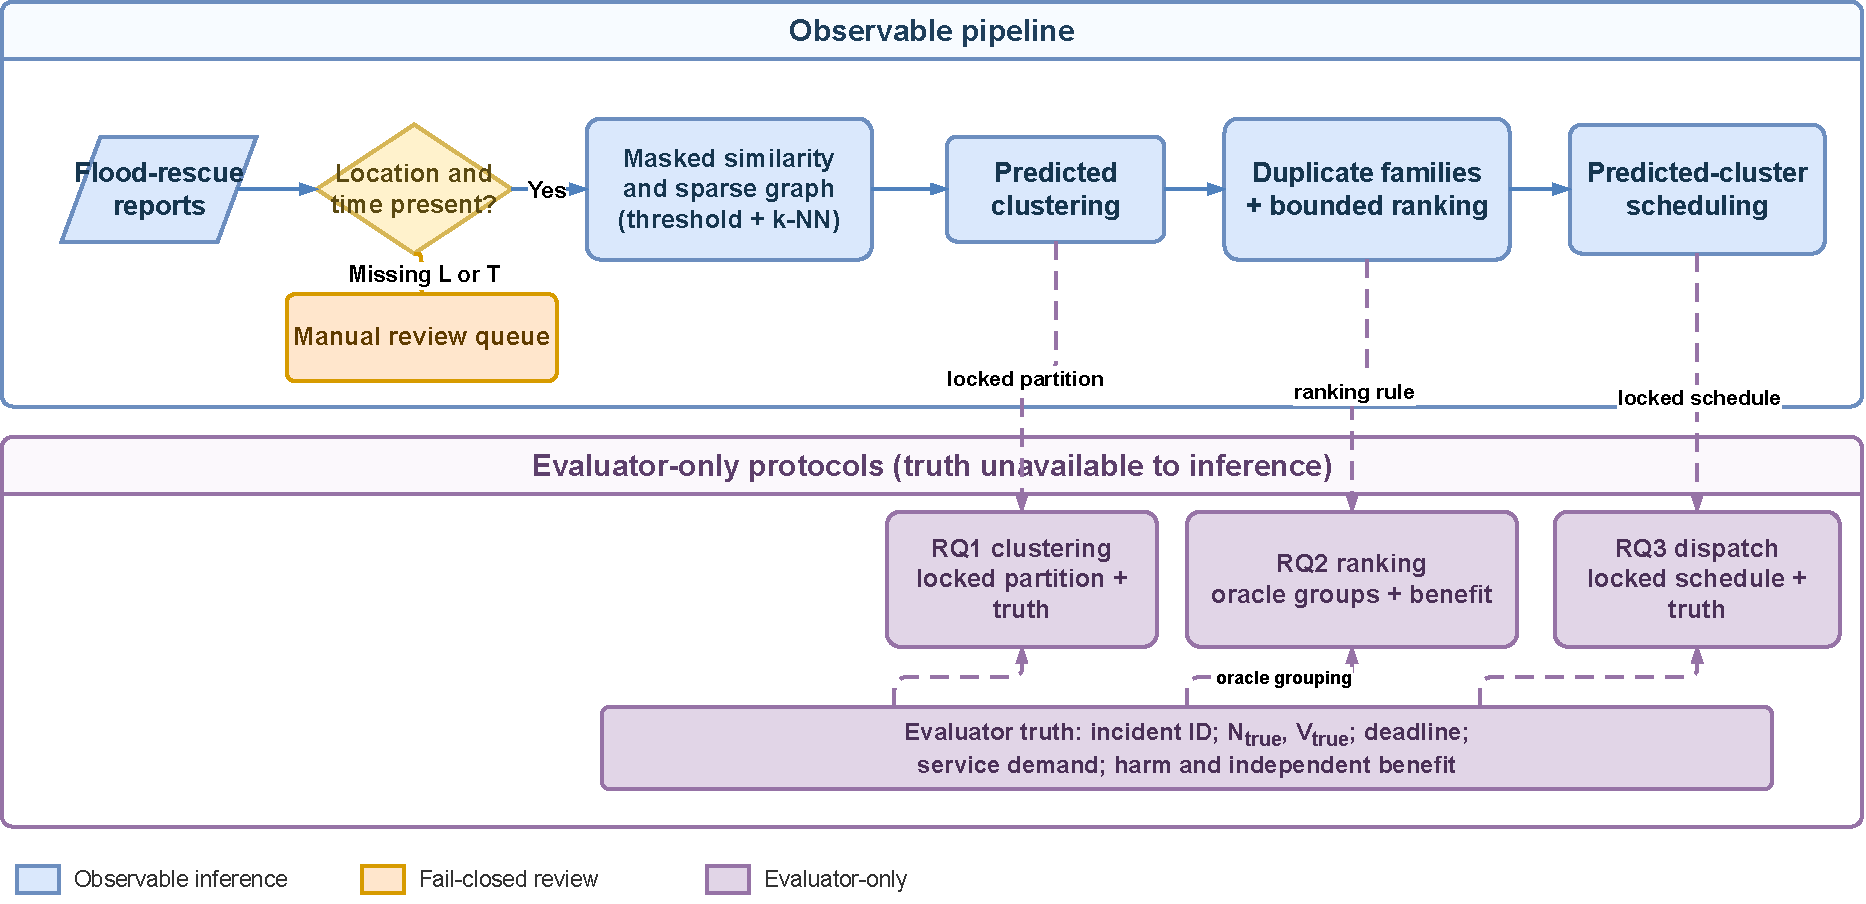
\includegraphics[width=\textwidth]{pipeline_v2.pdf}
\caption{Observable pipeline (solid), manual-review path (orange), and
evaluator-only truth join (dashed). The scheduler receives predicted clusters,
never incident truth.}
\label{fig:pipeline}
\end{figure}

\subsection{Missingness-Aware Similarity and Graph}

A report contains location $L_i$, event time $T_i$, flood evidence $F_i$,
urgency evidence $E_i$, reported demand $N_i$, vulnerability $V_i$, provenance
features, receipt time, and an observation mask. The graph admission indicator
$a_i$ is one only when $L_i,T_i$ are observed. Missing $F_i$ or $E_i$ is not
zero-imputed: let $I_F,I_E$ indicate pairwise shared observations and
$m_{ij}=I_F+I_E$; then
\[
C_{ij}=\frac{m_{ij}}{2}\exp\!\left[-I_F\frac{|F_i-F_j|}{\tau_F}
-I_E\frac{|E_i-E_j|}{\tau_E}\right],
\quad C_{ij}=0\ \text{if }m_{ij}=0.
\]
For Haversine distance $d_{ij}$ and time difference $\Delta t_{ij}$, define
\begin{align}
G_{ij}&=\exp[-d_{ij}^{2}/(2\sigma^2)],&
T_{ij}&=\exp[-\Delta t_{ij}/\tau_t],\nonumber\\
w^\times_{ij}&=a_i a_jG_{ij}(\beta T_{ij}+\gamma C_{ij}),&
w^+_{ij}&=a_i a_j(\alpha G_{ij}+\beta T_{ij}+\gamma C_{ij}).
\label{eq:similarities}
\end{align}
All scales $\sigma,\tau_t,\tau_F,\tau_E$ are strictly positive and the
weights are nonnegative. The implementation first forms a common spatial
candidate pool of at most $\max(64,4k)$ neighbours per eligible report,
including all boundary-distance ties before canonical truncation. It computes
an empirical nonzero-weight quantile, retains strict above-threshold edges,
keeps the union of endpoint-wise top-$k$ edges, and applies Louvain. Product
and additive candidates have the same pool and grid, but each family is
selected independently; the estimand is therefore a pipeline comparison, not
an operator-only causal effect.

\begin{theorem}[Product edge localization]
Let $B=\beta+\gamma>0$. If a product edge with threshold $0<\theta<B$ is
retained, then
$d_{ij}<\sigma\sqrt{2\log(B/\theta)}$. For $\theta\ge B$ the strict retained
set is empty; for $\theta\le0$ the threshold alone gives no finite cutoff.
\end{theorem}
\begin{proof}
Since $a_ia_j\le1$ and $T_{ij},C_{ij}\le1$,
$w^\times_{ij}\le B\exp[-d_{ij}^{2}/(2\sigma^2)]$. Combining
$\theta<w^\times_{ij}$ with positivity and taking logarithms gives the bound;
the endpoint cases follow from the same inequality.
\end{proof}
This is an edge statement. A component-diameter claim additionally needs a
bounded observed hop diameter; long transitive chains remain possible. For
the additive form, no general threshold-induced geographic cutoff exists when
$\theta\le\beta+\gamma$.

\subsection{Duplicate-Aware Bounded Ranking}

Provenance $Q_i\in[0,1]$ combines a source prior, image presence, and capped
corroboration from distinct source families; proximity alone cannot increase
it. Exact duplicates share a canonical fingerprint. Near duplicates are
merged by deterministic complete linkage, so $A\sim B\sim C$ does not merge
$A$ with $C$ unless every cross-pair passes the envelope.

Let $g$ index the resulting evidence families. Within each family, observed
fields are provenance-gated; across families, demand and vulnerability use
maxima rather than unsupported population sums. In compact form,
\begin{align}
\bar E&=\frac{\sum_g\max_{i\in g}Q_iE_i}
 {\max(1,\sum_g\max_{i\in g}Q_i)},&
\bar F&=\max_{g,i\in g}Q_iF_i,\nonumber\\
\bar N&=\min\!\left(1,\frac{\log(1+\max_{g,i\in g}Q_iN_i)}
 {\log(1+N_{\rm ref})}\right),&
\bar V&=\max_{g,i\in g}Q_iV_i,\nonumber\\
P&=\left[1+(\mu-1)\tanh(\bar V/s)\right]
 (\omega_E\bar E+\omega_F\bar F+\omega_N\bar N).
\label{eq:priority}
\end{align}
Claims are clipped before aggregation. We fix $\omega_E=.40$,
$\omega_F=.35$, $\omega_N=.25$, and $\mu=1.75$; hence
$0\le P\le1.75$. The weights and caps are policy knobs, not learned or
expert-validated parameters. Comparators are a multiplicity-sensitive legacy
score, urgency-only, population-only, a simple linear score, stable random,
and---for dispatch---nearest-first.

\section{Experimental Design}

\paragraph{Data contract and splits.}
At a predeclared 150-min receipt-time snapshot, reports received by the cutoff
are visible; late reports are excluded. A received report with missing event
time remains visible but enters review. ID data contain 16 authored incidents;
mechanism-shift OOD data vary incident count from 8 to 30 and change report
count tails, GPS noise and systematic bias, late order, source/severity-linked
missingness, contradictions, duplicates, campaigns, resources, and access
delays. Latent benefit is nonlinear, stochastic, and separate from
Eq.~\ref{eq:priority}. Seeds are disjoint: 20 development, 20 calibration, and
40 confirmation master seeds, each confirmation seed producing paired ID/OOD
datasets. Previously inspected seeds are explicitly retired.

\paragraph{Selection and comparators.}
Product and additive use the same 128-point nuisance grid:
$\sigma\in\{500,700,900,1200\}$ m, $\tau_t\in\{30,60\}$ min, quantile
$\in\{.85,.90,.95,.98\}$, $k\in\{8,16\}$, and resolution
$\in\{.8,1.2\}$, with fixed $\tau_F=.25,\tau_E=.35$ and
$\alpha=\beta=\gamma=.5$. ST-DBSCAN and geo-time HDBSCAN use complete
64- and 96-point grids. All 8,320 calibration executions succeeded. Within
each method, one rule maximizes mean ARI, retains the one-standard-error set,
then minimizes false destinations, maximizes noise rejection, minimizes review
burden, and breaks ties by canonical configuration ID.

\paragraph{Endpoints and inference.}
Clustering co-primary endpoints are ARI on incident-linked reports
~\cite{hubert1985comparing} and false destinations per 100 reports; noise
rejection and review items are secondary. Priority is scored on predicted
clusters before a one-to-one evaluator match supplies independent gains;
NDCG@5 is primary. Ten stress families cover exact, near, and gradual-chain
duplicates; four low-confidence fields; missingness; contradictions; and a
coordinated high-confidence nonincident campaign. For dispatch, each predicted
product cluster becomes a job; observable centroids, workloads, and three
resource scenarios determine the schedule. Truth joins afterward to measure
harm, missed deadlines, unreached incidents, false/duplicate trips, tail
response, and workload variation. Oracle grouping is a separate diagnostic
and never enters inference. Seed-paired effects use 10,000 bootstrap resamples,
paired Wilcoxon tests, and Holm adjustment within the frozen clustering and
priority/dispatch families. Positive effects always favour the revised
candidate; all adverse and null outcomes are retained.

\section{Results}

\ShortClusteringResultsTable

Table~\ref{tab:short-clustering-results} answers RQ1 negatively. Relative to
the independently selected additive pipeline, product ARI was lower by
$0.172$ (95\% CI $[-0.210,-0.136]$) on ID and $0.100$
($[-0.143,-0.058]$) on OOD data; Holm-adjusted $p<0.001$ in both cases.
The ID false-destination difference was inconclusive
($\Delta=-0.10$, $[-0.26,0.00]$), whereas OOD product clustering emitted
4.11 more false destinations per 100 reports
($\Delta=-4.11$, $[-6.06,-2.35]$, adjusted $p<0.001$). ST-DBSCAN and HDBSCAN
had descriptively higher OOD ARI and much lower false-destination rates than
product, but no registered inferential contrast against those baselines
supports a superiority statement. Every method lost ARI under mechanism shift.

\ShortPriorityDispatchResultsTable

Table~\ref{tab:short-priority-dispatch-results}, Panel A, also rejects a broad
RQ2 alignment claim. Revised NDCG@5 was below legacy by $0.092$ ID and $0.068$
OOD and was statistically indistinguishable from the simple linear score. It
beat population-only and random, but did not consistently beat urgency-only
after multiplicity correction. Exact duplicate injection nevertheless caused
zero revised-score drift in all 40 ID and 40 OOD datasets. That algebraic
success did not authenticate sources: the coordinated high-confidence
nonincident campaign produced the maximum false-priority lift, 1.0, in every
ID and OOD seed. Thus the duplicate-invariance gate passed, while the general
priority-alignment gate remained blocked.

Panel B propagates predicted clustering into RQ3. Against nearest-first, the
revised policy's improvement-oriented harm effect was $-33.57$
($[-47.88,-19.80]$) ID and $-30.88$ ($[-53.46,-7.95]$) OOD; deadline effects
were likewise adverse, $-0.137$ and $-0.075$. Revised ranking reduced harm
relative to population-only and random, but not relative to the strongest
simple policies. Across the predeclared family and guardrails, the
predicted-cluster dispatch-benefit gate therefore remained blocked. These
results would have been obscured by oracle incident grouping.

\section{Discussion and Threats to Validity}

The experiment separates mathematical safeguards from empirical benefit.
Product gating localizes retained edges, yet its independently selected
pipeline clustered worse than additive and direct density baselines in these
authored regimes. Because product and additive selected different nuisance
configurations, their contrast is not an isolated causal effect of
multiplication. Likewise, score boundedness and exact-duplicate invariance
limit numerical influence but do not defend against coordinated independent
sources; the campaign result is a concrete counterexample.

All reports, linkage, benefits, resources, and harms are synthetic. OOD changes
mechanisms rather than only seeds, but it remains an authored stress family.
An audit of planned public crisis and flood sources found no authorized dataset
with the joint physical linkage, rescue utility, and dispatch outcomes needed
for this evaluation; external, Vietnamese-transfer, real-clustering, and
real-dispatch gates remain blocked. No expert panel validated weights or caps.
The 150-min batch snapshot omits streaming adaptation, and travel, service, and
harm models simplify real access constraints. ST-DBSCAN/HDBSCAN comparisons
are descriptive, and the large locked Holm family is conservative. No result
supports ``deployment-ready'', misinformation robustness, or real-world harm
reduction.

\section{Artifact and Conclusion}

The accompanying artifact contains the frozen protocol, environment lock,
calibration selection, exact coverage manifests, aggregate analysis, tests,
and editable Figure~\ref{fig:pipeline}. The accepted manifest binds protocol,
implementation, selection, raw result, and analysis by SHA-256. The two tables
are generated only from the accepted analysis; the oracle artifact and
restricted public text are excluded.

In conclusion, the stress test found no product-clustering, general priority,
or predicted-dispatch advantage. Product ARI and OOD operational burden were
worse than additive; nearest-first outperformed revised dispatch on the main
comparisons. Exact-duplicate invariance held, but a coordinated campaign still
received maximal false priority. The defensible result is therefore a boundary:
edge localization and bounded ranking are useful audit properties, not evidence
of incident accuracy, policy validity, or rescue benefit.

\bibliographystyle{splncs04}
\bibliography{references}

\end{document}
